\newcommand{\ClassPath}{../../VIU_TFM_LaTeX_template}
\documentclass{\ClassPath/viu-tfm-template}
\usepackage{multicol}

\definecolor{maincolor}{HTML}{f25416}

%--------------------------------------------------------------------------
% Definiciones necesarias Modifica con tus datos
%--------------------------------------------------------------------------
\def\nombre{Gómez Olivencia, Rubén}
\def\dni{78910013-A}
\def\titulo{Biblioteca multimedia \linebreak\linebreak creada en Angular}
\def\titulacion{Máster Universitario en Desarrollo de Aplicaciones y Servicios Web}
\def\curso{2022-2023}

%Los siguientes son opcionales: si no se ponen, la portada cambia un poco. Ideal para escribir artículos/trabajos cortos
\def\dirige{}
\def\convocatoria{}
\def\asignatura{Desarrollo de aplicaciones web II: lado del cliente (front-end) y multimedia}


% importar fichero de Bibliografía
%\addbibresource{Actividad_1.bib}

\begin{document}
    \graphicspath{{../../VIU_TFM_LaTeX_template/}}

    \coverpage

    \tableofcontents

\chapter{Introducción}

A lo largo de este documento se van a explicar las decisiones tomadas, tanto en el ámbito de programación como de diseño, durante el desarrollo de una biblioteca multimedia (plataformas y series).

Para realizar este desarrollo se ha hecho uso del \textit{framework} de \textit{front-end} \href{https://angular.io/}{Angular}, que hace uso del lenguaje de programación \href{https://www.typescriptlang.org/}{Typescript}, y para dar un aspecto visual más cuidado se ha utilizado el \textit{framework} de estilos \href{https://getbootstrap.com/}{Bootstrap}.

\chapter{Finalizad del desarrollo}

La aplicación realizada es una biblioteca multimedia que contiene información acerca de las principales plataformas de Streaming que existen en la actualidad, con las series que se emiten en ellas y los actores/celebrities que participan en las mismas.

\begin{center}
    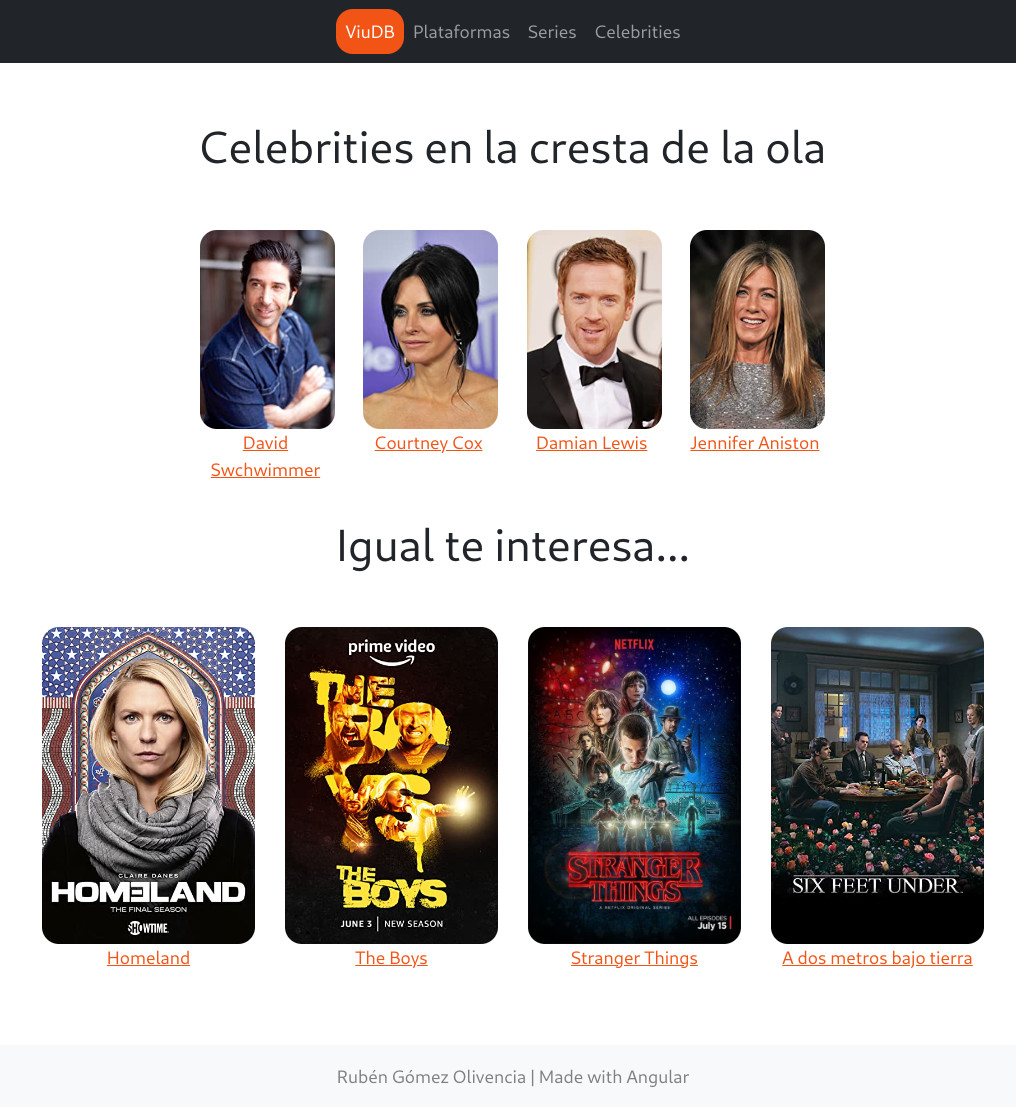
\includegraphics[frame,width=0.6\linewidth]{img/inicio.png}
\end{center}

No sólo vamos a poder visualizar la información de las distintas series, si no que también podremos visualizar el trailer de las mismas, y de esta manera saber si nos puede interesar empezar a ver la serie.

\chapter{Desarrollo realizado}
Tal como se ha indicado previamente, para realizar este proyecto se ha utilizado \href{https://angular.io/}{Angular} como \textit{framework} de desarrollo, por lo que vamos a diferenciar distintos aspectos utilizados en él.

\section{Uso de componentes}
Una de las características de Angular es la creación de componentes, para de esta manera poder crear separar la aplicación en distintos apartados que se pueden programar de manera separada, y tener su estilo propio.

Por ello, antes de comenzar con el desarrollo, se pensó cómo iba a ser el aspecto final de la aplicación y en cuántos componentes se iba a separar, así como la manera de poder reutilizarlos.

Si miramos, por ejemplo, la web de detalle de una plataforma, podemos diferenciar los siguientes componentes, que han sido diferenciados con distintos colores:

\vspace{-1em}
\begin{center}
    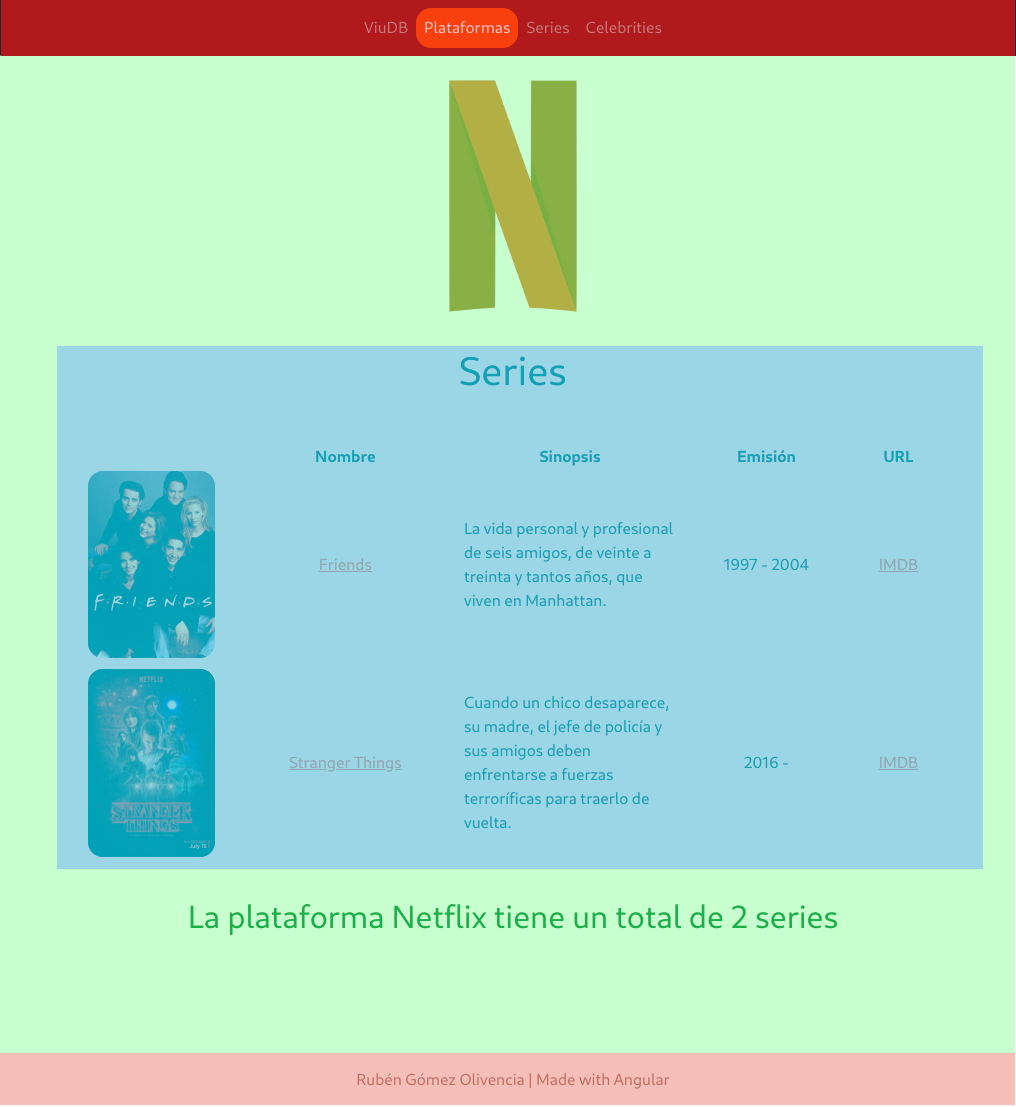
\includegraphics[frame,width=0.6\linewidth]{img/componentes.png}
\end{center}

\begin{itemize}
    \item \textbf{Cabecera}: La cabecera, o \textit{\textbf{navbar}}, nos permite ir a cualquiera de las secciones principales de la aplicación desde cualquier lugar de la misma, ya que siempre es visible. Nos indicará en qué sección estamos cambiando el color de la misma.

    \item \textbf{Sección principal}: Es donde se va a visualizar el contenido dinámico de la aplicación. Esta sección puede contener a su vez otros componentes. En este caso, se está utilizando el componente de series para mostrar únicamente las series que pertenecen a esta plataforma.

    \item \textbf{Pie de página}: También conocido como \textit{footer}, al igual que la cabecera, se muestra siempre. En este caso muestra el autor de la aplicación, pero en aplicaciones más complejas podría contener también enlaces a distintos apartados de la web, web de contacto, mapa de localización...
\end{itemize}

\section{Rutas y navegación}
Como la aplicación cuenta con distintas secciones principales, es conveniente que estas sean accesibles a través de distintas URLs para poder ser enlazadas. Es aquí donde entra en juego el \textbf{\textit{routing}}.

\begin{mycode}{Parte del fichero \textbf{app.routing.ts} }{typescript}{}
const appRoutes: Routes = [
  {path: '', component: InicioComponent},
  {path: 'plataformas', component: PlataformasComponent},
  {path: 'plataformas/:id', component: PlataformasShowComponent},
  {path: 'series', component: SeriesComponent},
  {path: 'series/:id', component: SeriesShowComponent},
  {path: 'celebrities', component: CelebritiesComponent},
  {path: 'celebrities/:id', component: CelebritiesShowComponent},
  {path: '**', component: ErrorComponent},
];
\end{mycode}

Tal como se puede ver en el código, se han creado ocho rutas distintas que harán uso de distintos componentes dependiendo de cuál sea la ruta seleccionada.

La selección del componente y la visualización del mismo se realiza gracias a la URL a la que accedamos y el apartado \inlineconsole{<router-outlet></router-outlet>} dentro del fichero \configfile{app.component.html}.

Es interesante destacar la última línea, ya que lo que indica es que si la URL de acceso no coincide con ninguna de las anteriores, lo que hará será visualizar el componente \textbf{ErrorComponent}, en el cual se ha indicado un mensaje de error.


\section{Paso de parámetros entre componentes}

Tal como se ha indicado previamente, la aplicación se ha realizado teniendo en cuenta las ventajas que nos permite el uso de componentes, y pensando en todo momento el que puedan ser reutilizados.

Esta reutilización se consigue pudiendo llamar desde un componente a otro y haciendo uso del paso de parámetros. De esta manera, podemos variar el comportamiento, y el aspecto, del componente dependiendo de cuál es el origen desde el que se le llama.

El ejemplo más claro es el componente \textbf{”series”}, que se encarga de obtener las series, dependiendo del lugar desde donde se le llama, y visualizarlas también de una manera distinta.

Este componente se reutiliza (y por tanto, recibe parámetros), desde tres sitios distintos:
\begin{itemize}
    \item \textbf{Página de inicio}: Se llama al componente con el parámetro “-1”, para de esta manera saber que se está llamando desde la página de inicio, y por tanto que visualice cuatro series de manera aleatoria y con aspecto horizontal.
    \vspace{-0.2em}
    \begin{center}
        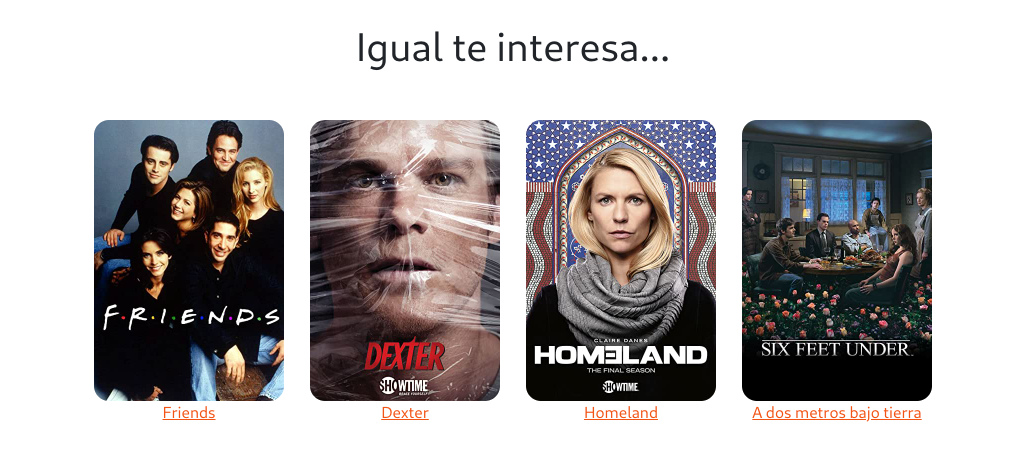
\includegraphics[frame,width=0.7\linewidth]{img/series-1.png}
    \end{center}

    \item \textbf{Sección “Series”}: Cuando se llama desde el menú principal, no se llama desde otro componente, por lo que el parámetro está inicializado a cero.

    En este caso nos visualiza todas las series con toda la información en formato tabla. Cada fila es una serie y cada columna tiene distinta información acerca de la misma.
    \vspace{-0.2em}
    \begin{center}
        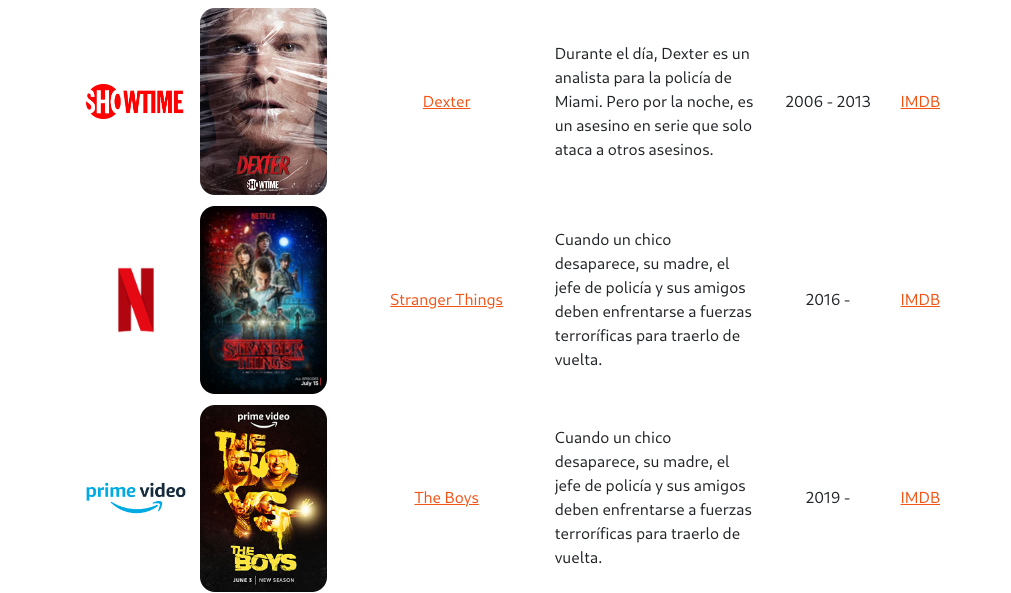
\includegraphics[frame,width=0.7\linewidth]{img/series-2.png}
    \end{center}

    \item \textbf{Información de una plataforma}: Al ir al detalle de una plataforma nos muestra todas las series de esa plataforma. Se llama al componente Series pasando como parámetro el identificador de la plataforma, para así sólo visualizar sus series.

    En este caso, el aspecto visual es similar al caso anterior, pero no se muestra la primera columna, que es la plataforma en el caso anterior, ya que quedaría redundante.

    \vspace{-0.2em}
    \begin{center}
        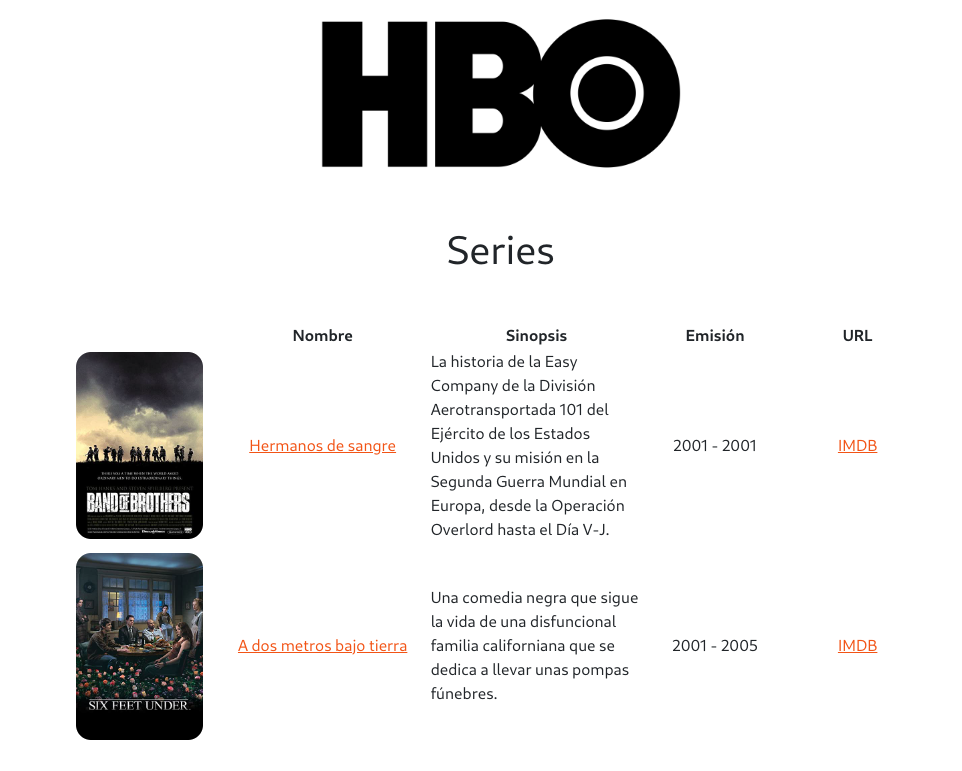
\includegraphics[frame,width=0.7\linewidth]{img/series-3.png}
    \end{center}
\end{itemize}


\subsection{Información del componente hijo al padre}
Hasta ahora se ha visto cómo un componente “hijo” recibe parámetros desde el componente “padre” que le llama. Pero la información también puede fluir en sentido contrario.

Esto se ha utilizado para mostrar el número de series que tiene una plataforma concreta, ya que es el componente hijo (componente “Series”) quien procesa la información y conoce el número de series, por lo que al terminar de mostrar la información y visualizarla, le envía al padre la información.

\begin{mycode}{Llamada al componente “\textbf{series}” desde “\textbf{plataformas-show}”}{html+ng2}{ {\small }}
<div>
    <app-series [plataforma_id]="plataforma.id"
                (series_count)="series_count=$event">
    </app-series>
</div>

<h2>La plataforma {{plataforma.nombre}}  tiene un total de {{series_count}}
    {{series_count>1?"series":"serie"}}</h2>
\end{mycode}

En el código expuesto, se puede ver cómo se llama al componente “series” pasando el parámetro “plataforma\_id” para que sepa qué series tiene que mostrar. A su vez, del componente recibiremos información a través de un evento que guardaremos en la variable \inlineconsole{series_count} para después visualizarla.



\chapter{Dificultades del proyecto}

Como todo proyecto de programación, durante el desarrollo nos podemos encontrar con ciertas dificultades que deben ser subsanadas para llegar a cumplir los requisitos planteados al comienzo del proyecto.


\chapter{Conclusiones}

A la hora de afrontar un proyecto, aunque el algoritmo generado pueda ser sencillo, no quita que exista un proceso de aprendizaje a la hora de utilizar ciertas herramientas no conocidas.



\end{document}
